%*******************************************************
% Anti-Aliasing
%*******************************************************
\section{Anti-Aliasing}

To support anti-aliasing the optional \verb|<aa_samples>| parameter was added to
the \verb|gr.render| Lua command.

The parameter specifies the number of rays to cast per pixel. By default this
parameter is set to one.

Anti-aliasing is implemented using stratified super-sampling where the pixel is
divided into a $n\times n$ grid and a ray is cast from a random point within 
each grid box as shown in Figure~\ref{fig:image1} (Shirley \& Marschner, 2009).

\begin{figure}[ht]
  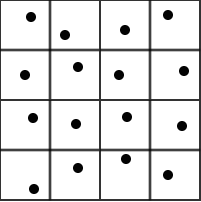
\includegraphics[width=0.5\textwidth, center]{stratified_sampling}
  \caption{Illustration of how samples are distributed within a pixel in 
  stratified sampling}
  \label{fig:image1}
\end{figure}

Stratified sampling different from uniform sampling and jittered 
sampling (see Figure~\ref{fig:image2}). Stratified sampling is preferred over 
both uniform and jittered sampling since uniform sampling can not minimize the 
effects of regular artifacts since sampling is done at regular intervals within 
the pixels and jittered sampling has the problem of introducing clumping of 
samples in one area within the pixel.

\begin{figure}[ht]
\begin{subfigure}{0.5\textwidth}
  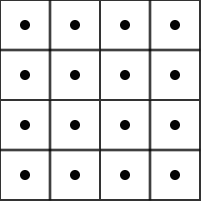
\includegraphics[width=0.5\linewidth, center]{uniform_sampling}
  \caption{Uniform Super-Sampling}
  \label{fig:subim1}
\end{subfigure}
\begin{subfigure}{0.5\textwidth}
  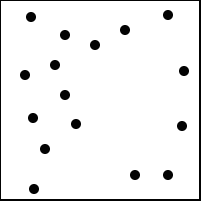
\includegraphics[width=0.5\linewidth, center]{jittered_sampling}
  \caption{Jittered Super-Sampling}
  \label{fig:subim2}
\end{subfigure}
\caption{Diagrams illustrating how samples are distributed within a pixel for
the uniform and jittered sampling methods}
\label{fig:image2}
\end{figure}

